\documentclass[11pt]{article}

\usepackage{titlesec}
\usepackage[hidelinks]{hyperref}
\usepackage{titling}
\usepackage[margin=1in,headheight=0pt,headsep=0pt]{geometry}
\usepackage{multicol}
\usepackage{graphicx}
\usepackage{tcolorbox}
\usepackage{multirow}
\usepackage{makecell}
\usepackage{xcolor}
\usepackage{titlesec}
\usepackage{pifont} % bullet points for itemize
\usepackage{enumitem} % packed itemize


\definecolor{mycolor}{rgb}{0.122, 0.435, 0.698}% Rule colour

% Reduce the margin from the top of the page
\setlength{\voffset}{-0.0in}
\setlength{\headsep}{5pt}

\pagestyle{empty} 

% Format some parts
\titleformat{\section}
{\Large\bfseries\uppercase}
{}
{0em}
{}[\titlerule]

\titleformat{\subsection}
{\bfseries\Large}
{$\bullet$}
{0em}
{}

\titleformat{\subsubsection}
{\bfseries}
{}
{0em}
{}

\newtcbox{\topic}{on line,
colframe=mycolor,
colback=mycolor!10!white,
boxrule=0.5pt,
arc=4pt,
boxsep=0pt,
left=6pt,
right=6pt,
top=6pt,
bottom=6pt}

\newtcbox{\nameTitleBox}{on line,
colframe=gray,
colback=white,
boxrule=1pt,
arc=2pt,
boxsep=0pt,
left=6pt,
right=6pt,
top=6pt,
bottom=6pt}

% define function
% arguments: level, place, graduation, image
\newcommand*{\eduWithDetail}[5]
{\begin{table}[h!]
	\begin{tabular*}{\textwidth}{ll@{\extracolsep{\fill}}r}
		\textbf{#1} &  #2 & \\ % \multirow{2}{*}{\includegraphics[width=40px]{#4}} \\
		#3 &  & \\
		\multicolumn{3}{l}{#5}
	\end{tabular*}
\end{table}}

\newcommand*{\eduSmall}[5]
{\begin{table}[h!]
	\begin{tabular*}{\textwidth}{ll@{\extracolsep{\fill}}r}
		\textbf{#1} &  #2 & \\ % \multirow{2}{*}{\includegraphics[width=40px]{#4}} \\
		#3 &  & \\
		\multicolumn{3}{l}{#5}
	\end{tabular*}
\end{table}}

\newcommand*{\multilineCell}[1]
{\begin{tabular}[c]{@{}l@{}} #1
\end{tabular}}

% 1: Name 2: Date 3: Lecturer 4: Level
\newcommand*{\taRecord}[4]{\textbf{#1}\quad (#3) \\ #2 \quad  #4}

\def\today{\number\day \space \ifcase\month\or
	Jan\or Feb\or Mar\or Apr\or May\or Jun\or
	Jul\or Aug\or Sep\or Oct\or Nov\or Dec\fi
	\space \number\year}


\usepackage{paracol}
\usepackage[bottom]{footmisc}
\usepackage{colortbl}
\usepackage{lipsum}
\usepackage{setspace}
\usepackage{amssymb}
\usepackage{soul}

\usepackage{hyperref}
\RequirePackage{fontawesome}

\usepackage{fontawesome}
\usepackage{setspace}

\begin{document}
	

	
% Title and Header section
% {% Image
%     \begin{minipage}[t]{100px}
%         % add a row so that contacts minipage is alligned with
%         % this line, but remove the space added for the line
%         \strut\vspace*{-\baselineskip}\newline
%         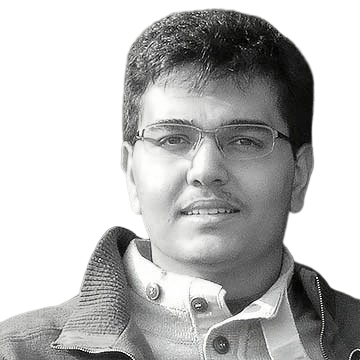
\includegraphics[width=80px]{images/farbod.png} \\
%     \end{minipage}
%     Name
%     \nameTitleBox{
%     \begin{minipage}[t]{3.5cm}
%         \vspace{8mm}
%         \noindent
%         \huge\bfseries
%         Farbod\\
%         Shahinfar
%         % \vspace{0.0cm}
%     \end{minipage}
%     }
%     \hfill\null
%     \begin{minipage}[t]{6cm}
%         \vspace{6mm}
%         % Contact Information
{ % \small
% \noindent
% \flushright
\noindent
% Phone: +989128077968 \\
\small \faEnvelope  \hspace{0.05cm}   Email: \href{mailto:iman.rahmati@sharif.edu}{iman.rahmati@sharif.edu} \space \href{mailto:imanrht@gmail.com}{imanrht@gmail.com} \\
%\faLink \hspace{0.05cm} Web page: \href{https://imanrht.github.io}{imanrht.github.io} \\
\faGithub \hspace{0.1cm} Github: \href{https://github.com/ImanRHT}{https://github.com/ImanRHT}  \\
\faLinkedin \hspace{0.1cm} Linkedin: \href{https://linkedin.com/in/iman-rahmati}{linkedin.com/in/iman-rahmati}\\
% Birthday: 25/Feb/1998 \\
}
% ===================================================================

%     \end{minipage}
% }
{\noindent \huge\bfseries Iman Rahmati}\hfill%{\footnotesize updated: \today}
\vspace{-1cm}
\section{}
% Contact Information
{ % \small
% \noindent
% \flushright
\noindent
% Phone: +989128077968 \\
\small \faEnvelope  \hspace{0.05cm}   Email: \href{mailto:iman.rahmati@sharif.edu}{iman.rahmati@sharif.edu} \space \href{mailto:imanrht@gmail.com}{imanrht@gmail.com} \\
%\faLink \hspace{0.05cm} Web page: \href{https://imanrht.github.io}{imanrht.github.io} \\
\faGithub \hspace{0.1cm} Github: \href{https://github.com/ImanRHT}{https://github.com/ImanRHT}  \\
\faLinkedin \hspace{0.1cm} Linkedin: \href{https://linkedin.com/in/iman-rahmati}{linkedin.com/in/iman-rahmati}\\
% Birthday: 25/Feb/1998 \\
}
% ===================================================================
 \vspace{-2mm}

\noindent{\textbf{Research Interests:}} Distributed Systems, Mobile Edge Computing (MEC), Multi-Agent Deep Reinforcement Learning (DRL), Federated/Distributed Learning, Performance Evaluation
\vspace{-3mm}
\section{Education}



%\vspace{-0.5cm}
%\eduWithDetail{Ph.D. Information Technology}
%{Politecnico di Milano}
%{Expected Graduation date 2026}
%{}
%{\multilineCell
%	{\hspace{5mm} \textbf{Advisor}: Prof. Gianni Antichi}
%}
\vspace{-5mm}
%COMPUTER NETWORKS ENGINEERING/
\eduWithDetail{MSc. Computer Engineering/Networking}
{\hspace{1.2cm} Sharif University of Technology (SUT)}
{Graduated Sep 2022, 4/4 GPA}
{images/sharif.png}
{\multilineCell
	{
        \hspace{5mm} \textbf{Thesis Title}:
        A decentralized resource allocation algorithm utilizing DRL for MEC, \\ \hspace{31mm} aimed at optimizing latency and energy efficiency. \\ %\href{https://github.com/ImanRHT/Master_Thesis}{\faGithub}\\
        \hspace{5mm} \textbf{Supervisor}: Prof. Ali Movaghar \href{https://scholar.google.com/citations?user=BXNelwwAAAAJ\&hl=en}{\small \faExternalLink}}
}
\vspace{-5mm}    


\eduWithDetail{BSc. Industrial Engineering}
{\hspace{1.3cm}Khajeh Nasir Toosi University of Technology (KNTU)}
{Graduated Sep 2019}
{images/iust.png}
{%\multilineCell{\hspace{5mm}\vspace{-3mm} \\ %\textbf{Frist Rank}, 18.62/20 GPA \\
	%\hspace{5mm} \textbf{Project}:
	%Study of MMU Cache Partitioning Efficacy for Hierarchical Page Tables \\
	%\hspace{10mm} in OS Memory Management \\
	%\hspace{5mm} \textbf{Supervisor}: Dr. Mohsen Sharifi}
}
\vspace{-10mm}

% \eduSmall{High School Diploma}
% {Salam 3}
% {Graduated May 2015}
% {images/salam.png}
% {\hspace{5mm} \textbf{GPA:} 19.84/20}





\section{Academic Experience}


\large{\textbf{Research Engineer at EdgeAI Lab} } \hfill 2022-Present\vspace{1mm}
\normalsize

	\hspace{-5.5mm}Supervisor: Prof. {Hamed Shah-Mansouri} \href{https://scholar.google.com/citations?user=dcjIFccAAAAJ&hl=en&oi=ao}{\small \faExternalLink} \href{https://scholar.google.com/citations?user=BXNelwwAAAAJ\&hl=en}\hfill Department of Electrical Engineering, SUT
	\begin{itemize}
		\vspace{-2mm}  
		\item\textbf{Research Theme:} Developing hierarchical multi-agent DRL-based approaches for computation offloading decision-making in heterogeneous MEC, with an emphasis on centralized training and decentralized execution to achieve collaborative global optimization.\\ 
	\end{itemize}
\vspace{-5mm}
\large{\textbf{Research Assistant at Performance and Dependability Lab (PDL)} }\hfill 2019-2022\vspace{1mm}

\normalsize
\hspace{-5.5mm}Supervisor: Prof. \href{https://scholar.google.com/citations?user=BXNelwwAAAAJ\&hl=en}{Ali Movaghar} \hfill Department of Computer Science and Engineering, SUT\vspace{-2mm}
\begin{itemize}
	\item\textbf{Research Theme:} Developing DRL-based algorithms to optimize computation offloading decisions in MEC, with a primary focus on enhancing the quality of experience (QoE) for end-users of mobile applications.
\end{itemize}
\large\large\textbf{Teaching Assistant}  \vspace{-2mm}
\normalsize

\begin{itemize}
	


	\item \textbf{Performance Evaluation of Computer Systems (Head TA)} \hfill SUT, 2020-2022
		\\ Prof. Ali Movaghar and Dr. Mahdi Dolati \vspace{-2mm} \href{https://scholar.google.com/citations?user=b7A2CXYAAAAJ&hl=en&oi=ao}{\small \faExternalLink}
	\item \textbf{Software Defined Networking (Head TA)} \hfill SUT, 2022
		\\ Prof. Ali Movaghar and Dr. Mohammad Hosseini \vspace{-2mm} \href{https://scholar.google.com/citations?user=iRO-DVoAAAAJ&hl=en&oi=ao}{\small \faExternalLink}
	\item \textbf{Verification of Reactive Systems} \hfill SUT, 2021
		\\ Prof. Ali Movaghar \vspace{-2mm}
			\item \textbf{Wireless Networking} \hfill SUT, 2021
	\\ Prof. Ali Mohammad Afshin Hemmatyar \vspace{-2mm} \href{https://scholar.google.com/citations?user=wob0AskAAAAJ&hl=en&oi=ao}{\small \faExternalLink}
	\item \textbf{Theory of Machines and Languages} \hfill SUT, 2021
		\\ Prof. Ali Movaghar \vspace{-2mm}

		

\end{itemize}

\hspace{-7mm}\textbf{Sub-Reviewer at 27th International Computer Conference}\hfill CSICC, 2022 \\
  \textcolor{white}{iiiiiii}Computer Society of Iran (CSICC) \href{http://csi.org.ir/csicc2022/index-2.html}{\small \faExternalLink}\\ \textcolor{white}{iiiiii} IEEE website published papers from this conference. \href{https://ieeexplore.ieee.org/xpl/conhome/9780464/proceeding}{\small \faExternalLink}
  
  
  \section {Publication}
  
  \begin{itemize}
  	
  	\item I. Rahmati, H. Shah-Mansouri, A. Movaghar, ``QECO: A QoE-Oriented Computation Offloading Algorithm based on Deep Reinforcement Learning for Mobile Edge Computing'', Accepted in IEEE Transactions on Network Science and Engineering, 2024.
  	\href{https://arxiv.org/pdf/2311.02525}{\small  \faExternalLink}
  	\href{https://github.com/ImanRHT/QECO}{\faGithub}
  	
  	
  	\item I. Rahmati, H. Shah-Mansouri, H. Kebriaei, A. Movaghar, "Multi-Agent Deep Reinforcement Learning for Energy-Efficient Cooperative Computation Offloading in Heterogeneous Mobile Edge Computing," work in progress.
  	
  	\item I. Rahmati, A. Movaghar, "Federated Deep Reinforcement Learning Improves Dependent Task Offloading in Mobile Edge Computing'', work in progress.
  	

  \end{itemize}

\section{Honors}
\begin{itemize}
	\renewcommand\labelitemi{\ding{118}}
	\item{Ranked in the top 10\% of M.Sc. students in the Department of Computer Engineering at SUT, Class of 2019  \hfill  2022}\vspace{-2mm}
	\item {Ranked 55$^{th}$ among 60,000 participants in the Nationwide University Entrance Exam of Computer Engineering for M.Sc. in the field of Networking \hfill  2019}\vspace{-2mm}
	\item{Ranked Top 1\% among 180,000 participants in the Nationwide University Entrance Exam for B.Sc. in the field of Mathematics and Physics  \hfill  2014}\vspace{-2mm}
	\item{Achieving the 3$^{th}$ position in the RoboCup Competition (IranOpen)  \hfill  2012}\vspace{-2mm}
\end{itemize}


\section{Academic Projects}

\begin{itemize}
	

		
	%\item \textbf{QoE Maximization in Mobile Edge Computing} \hfill SUT, 2022\\
	%Optimizing Decision-Making for Computation Offloading in Mobile Edge Computing using Deep Reinforcement Learning (Dueling Deep Q-Networks) \href{https://github.com/ImanRHT/QECO}{\faGithub} \\Supervisor: Prof.  Ali Movaghar and Prof. Hamed Shah-Mansouri \href{https://scholar.google.com/citations?user=dcjIFccAAAAJ&hl=en&oi=ao}{\small \faExternalLink} 
	
	
	\item \textbf{Multi-Agent Deep Deterministic Policy Gradiant Networks} \hfill EdgeAI, 2023\\
	Designed based on decentralized partially observable markov decision processes (Dec-POMDP) and employed for computation offloading in heterogeneous MEC.
	
	
	
	\item \textbf{Dueling Double Deep Q-Networks (D3QN)} \hfill PDL, 2022\\
     Designed based on markov decision processes and employed for distributed computation offloading decision-making. \href{https://github.com/ImanRHT/QECO}{\faGithub} %\href{https://github.com/ImanRHT/QECO}{\faGithub} %\\Supervisor: Prof.  Ali Movaghar and Prof. Hamed Shah-Mansouri \href{https://scholar.google.com/citations?user=dcjIFccAAAAJ&hl=en&oi=ao}{\small \faExternalLink} 
	
	
	\item \textbf{Mobile Edge Computing Environment} \hfill PDL, 2021\\
	Modeled and simulated resource-constrained MEC for latency and energy optimization. \href{https://github.com/ImanRHT/MEC_Environment}{\faGithub} %Supervisor: Prof.  A. Movaghar and Dr. H. Shah-Mansouri
	

	
	\item \textbf{Long Short Term Memory} \hfill PDL, 2021\\
	Designed and modeled for forecasting edge servers' workload based on time series analysis.
	%\href{https://github.com/ImanRHT/Tiime_Series_Prediction}{\faGithub} Supervisor: Prof.  Ali Movaghar
	
	
	\item \textbf{Queueing System} \hfill SUT, 2020\\
	Discrete event simulation and performance evaluation of M/M/1/K queues with various service disciplines. \href{https://github.com/ImanRHT/MM1K_Queue_Simulation}{\faGithub} 
	


%	\item \textbf{Distributed Systems} \hfill SUT, 2019\\
%	A Survey on `Verification of Paxos and Raft Protocols in Distributed Consensus’ \\
%	Supervisor: Prof. Mohammad Izadi	\href{https://scholar.google.com/citations?user=On8Cw-MAAAAJ&hl=en&oi=ao}{\small \faExternalLink}

%	\item \textbf{Production Planning Optimization} \hfill KNTU, 2017\\
%Maximizing profit involves determining the optimal quantity of each product to produce, taking into account production costs and demand.\\
%Supervisor: Prof. Amir Abbas Najafi
%\href{https://scholar.google.com/citations?user=adOQSIEAAAAJ&hl=en&oi=ao}{\small \faExternalLink}

%	\item \textbf{Decision Making Analysis} \hfill KNTU, 2018\\
%	A survey on ’Application of Data Envelopment Analysis (DEA) for Evaluating Efficiency by MATLAB’\\ 
%	Supervisor: Dr. Naser Safaie
%	\href{https://scholar.google.com/citations?user=J0M--CIAAAAJ&hl=en&oi=ao}{\small \faExternalLink}
	
%	\item \textbf{Driving Simulation} \hfill KNTU, 2018\\
%	Analysis and evaluation of nervous and excitement body system reactons, Facing critical driving situations in Python,\\
%	Supervisor: Dr. Donya Rahmani
%	\href{https://scholar.google.com/citations?user=qUqJT7MAAAAJ&hl=en&oi=ao}{\small \faExternalLink}
	

	
%	\item \textbf{Quality Management} \hfill KNTU, 2017\\
%	Implementation of Failure Modes and Effects Analysis (FMEA) from a Managerial Perspective\\
%	Supervisor: Dr. Naser Safaie
	
\end{itemize}




\section{SELECTED COURSES}
		\vspace{-5mm}
	     \setlength\itemsep{0em}
	     \begin{multicols}{2}
				- Theory of Distributed Systems  \hfill $4/4$ 
				
			    -  Computer Performance Evaluation \hfill $4/4$
			    
			    - Verification of Reactive Systems  \hfill  $4/4$
			     
				 - Advanced Network Security  \hfill $4/4$
				 
		         - Wireless Networking  \hfill $4/4$
		         
		         - Computer Network  \hfill $4/4$
		         
		          - IT Enterprise architecture  \hfill  $4/4$
		         
		         - Computer Network Management  \hfill $3.9/4$
		         

		         
		         % \item {C\#}
		         % \item {Java}
		         % \item {SQL}
		     \end{multicols}


\section{Skills}



\begin{itemize}[noitemsep,topsep=0pt,parsep=0pt,partopsep=0pt]
	\item {\textbf{General:} Networking, MEC, Multi-Agent DRL, Simulation, Performance Evaluation}\vspace{1mm}
	\item {\textbf{Programming Languages:} Python, R, Bash, C++}\vspace{1mm}
	\item {\textbf{Machine Learning:} TensorFlow, PyTorch, Scikit-learn}\vspace{1mm}
	\item {\textbf{Data Analysis:} Pandas, NumPy, Matplotlib}\vspace{1mm}
	\item {\textbf{Frameworks \& Tools:} Linux, Mininet, Ns-3, Git, \LaTeX, Vim, Flask, Visio}\vspace{1mm}
	\item {\textbf{Language Proficiency:} Farsi (Native), English (Working proficiency)}\vspace{1mm}\\
	- TOEFL (IBT) Score: 108/120 (R: 30, L: 28, S: 22, W: 28)


\end{itemize}


\section{CERTIFICATION}  

\textbf{Interactive Learning}  \hfill Tehran Institute for Advanced Studies (TeIAS), 2021\\
Certification of Completion in Deep Reinforcement Learning Course, Inst: Prof. Majid Nili	\href{https://scholar.google.com/citations?user=QlwWxmoAAAAJ&hl=en}{\small \faExternalLink}\\
\textbf{Machine Learning and Deep Learning in Python}  \hfill Start-Tech Academy, 2020\\
Certification of Completion in Udemy Online Course\\
\textbf{Data Science} \hfill Tose’e Higher Education Institute, 2019\\
Certification of Completion in Data Science Course, Inst: Dr. Yaser Zerehsaz \href{https://scholar.google.com/citations?user=QlwWxmoAAAAJ&hl=en}{\small \faExternalLink}\\
\textbf{Advanced Python Topics} \hfill Remis Arjang Institute, 2018\\
Certification of Completion in Advanced Python Course, Inst: Dr. Peyman Hooshmandi\\
\textbf{LPIC1} \hfill Anisa Iran Linux House, 2017\\
Certification of Completion in Linux Administrator Course, Inst: Dr. Amir Abbasi

\section{REFERENCES}

\textbf{Prof. Ali Movaghar} \href{https://scholar.google.com/citations?user=BXNelwwAAAAJ\&hl=en}{\small \faExternalLink} \hfill movaghar@sharif.edu\\
Professor of Computer Science and Engineering Department, SUT \\
Visiting Professor of Computer Science Department, University of Michigan\\
\textbf{Prof. Hamed Shah-Mansouri} \href{https://scholar.google.com/citations?user=dcjIFccAAAAJ&hl=en&oi=ao}{\small \faExternalLink} \hfill  hamedsh@sharif.edu\\
Assistant Professor of Electrical Engineering Department, SUT\\
\textbf{Prof. Ali Mohammad Afshin Hemmatyar} \href{https://scholar.google.com/citations?user=wob0AskAAAAJ&hl=en&oi=ao}{\small \faExternalLink}  \hfill hemmatyar@sharif.edu\\
Professor of Computer Science and Engineering Department, SUT\\
%\textbf{Dr. Mohammad Hosseini} \href{https://scholar.google.com/citations?user=iRO-DVoAAAAJ&hl=en&oi=ao}{\small \faExternalLink} \hfill  \href{mailto:hosseini@ipm.ir}{hosseini@ipm.ir} \\ Postdoctoral of Institute For Research In Fundamental Sciences Researcher (IPM)\\
%\textbf{Dr. Mahdi Dolati} \href{https://scholar.google.com/citations?user=b7A2CXYAAAAJ&hl=en&oi=ao}{\small \faExternalLink} \hfill  \href{mailto:mahdidolati@ut.ac.ir}{mahdidolati@ut.ac.ir}\\ Postdoctoral of Institute For Research In Fundamental Sciences Researcher (IPM)\\
\vfill
Further information are available upon Request.

\end{document}
